% Filename  : samplepaper.tex
% Purpose   : A sample exam paper to demonstrate how to use the 'ditpaper'
%             TeX class.
% Author    : Emmet Caulfield
% Revision  : $Id: samplepaper.tex 2 2006-02-19 20:34:45Z emmet $
% Repository: $HeadURL: http://svn.netrogen.lan/tex-ditpaper/trunk/samplepaper.tex $
%

% 'nosolution' (default) and 'solution' toggle the inclusion of solutions
% in the output. The tag solution, below, is replaced by 'sed' 
% in the Makefile to cause both the paper and the solutions to be produced.
%\documentclass[solution]{ditpaper}

\documentclass[solution]{ditpaper}
%\documentclass[solution]{ditpaper}

%\usepackage{epsf}
\usepackage{fleqn}
%\usepackage{rotating}
\usepackage{graphicx}


%%%%%%%%%%%%%%%%%%%%%%%%%%%%%%%%%%%%%%%%%%%%
%% Start newcommand defs taken from aima slides style file %%%%%%%%%%%%%%
%%%%%%%%%%%%%%%%%%%%%%%%%%%%%%%%%%%%%%%%%%%%

\def\mysum{\begin{Huge}\mbox{$\Sigma$}\end{Huge}}
\def\myint{\begin{LARGE}\mbox{$\int$}\end{LARGE}}
\def\myprod{\begin{Huge}\mbox{$\Pi$}\end{Huge}}

\newcommand{\smbf}[1]{\mbox{{\smathbold #1}}}
\newcommand{\mbf}[1]{\mbox{{\bf #1}}}

%%%%%% logical symbols
\newcommand{\entails}{\models}
\newcommand{\implies}{\:\;{\Rightarrow}\:\;}
\newcommand{\textimplies}{\;{\Rightarrow}\;}
\newcommand{\impliessymbol}{\Rightarrow}
\newcommand{\lequiv}{\;\;{\Leftrightarrow}\;\;}
\newcommand{\textlequiv}{\;{\Leftrightarrow}\;}
\newcommand{\lequivsymbol}{\Leftrightarrow}
\newcommand{\xor}{\not\lequiv}
\newcommand{\All}[1]{\forall\,#1\;\;}
\newcommand{\Exi}[1]{\exists\,#1\;\;}
\newcommand{\Exii}[1]{\exists!\,#1\;\;}% -pnorvig
\newcommand{\Iot}[2]{\iota\,#1\,#2}
\newcommand{\Lam}[2]{\lambda #1\;#2}
\newcommand{\Qua}[3]{[#1\,#2\;#3]}

\newcommand{\union}{{\,{\cup}\,}}
\newcommand{\intersection}{{\,{\cap}\,}}
\renewcommand{\emptyset}{\{\,\}}
\newcommand{\emptylist}{[\,]}
\newcommand{\adjoin}[2]{\{#1|#2\}}
\newcommand{\elt}{{\,{\in}\,}}  %%%cuts down on spacing
\newcommand{\eq}{{\,{=}\,}}  %%%cuts down on spacing
\def\stimes{{\,\times\,}}       %%%cuts down on spacing

\newcommand{\sr}[1]{\mathrel{\raisebox{-0.6ex}{$\stackrel{#1}{\longrightarrow}$}}}
\newcommand{\srbox}[1]{\sr{\fboxsep=1pt\fbox{$\,{\scriptstyle #1}\,$}}}
\newcommand{\srboxbox}[1]{\sr{\fboxsep=1pt\fbox{\fbox{$\,{\scriptstyle #1}\,$}}}}

\def\Diff{\mbox{{\it Diff}}}

%%%%%% probability and decision theory
\newcommand{\pv}{\mbf{P}}
\newcommand{\qv}{\mbf{Q}}
\newcommand{\given}{\mid}
\def\transition#1#2{q(#1\rightarrow #2)}
\newcommand{\otherthan}{\overline}
\newcommand{\Parents}{Parents}
\newcommand{\parents}{parents}
\newcommand{\Children}{Children}
\newcommand{\children}{children}
\newcommand{\MarkovBlanket}{MB}
\newcommand{\markovBlanket}{mb}

\def\X{\mbf{X}}
\def\x{\mbf{x}}
\def\sx{\smbf{x}}
\def\Y{\mbf{Y}}
\def\y{\mbf{y}}
\def\sy{\smbf{y}}
\def\E{\mbf{E}}
\def\e{\mbf{e}}
\def\D{\mbf{D}}
\def\d{\mbf{d}}
\def\sbe{\smbf{e}}
\def\sE{\smbf{E}}
\def\T{\mbf{T}}
\def\O{\mbf{O}}
\def\se{\smbf{e}}
\def\Z{\mbf{Z}}
\def\z{\mbf{z}}
\def\sz{\smbf{z}}
\def\F{\mbf{F}}
\def\f{\mbf{f}}
\def\A{\mbf{A}}
\def\B{\mbf{B}}
\def\C{\mbf{C}}
\def\b{\mbf{b}}
\def\m{\mbf{m}}
\def\I{\mbf{I}}
\def\H{\mbf{H}}
\def\zeroes{\mbf{0}}
\def\ones{\mbf{1}}
\def\ev{\mbf{ev}}
\def\fv{\mbf{ev}}
\def\sv{\mbf{sv}}

%%%%%%%%%%%%%%%%%%%%%%%%%%%%%%%%%%%%%%%%%%%%
%% End newcommand defs taken from aima slides style file %%%%%%%%%%%%%%
%%%%%%%%%%%%%%%%%%%%%%%%%%%%%%%%%%%%%%%%%%%%





% These must be set or bizarre defaults will be used:
\facility{Kevin Street, Dublin 8}
\course{BSc. (Hons) in Computer Science}
\examcode{S228/419C}
\stage{Stage 4}
\session{Semester 2 Examinations 2013/2014}
\title{Artificial Intelligence II}
\examiners{Dr. John Kelleher\\
Dr. Deirdre. Lillis\\
Mr. P. Collins}
\examdate{Monday\\$12^{th}$ May 2014}
\examtime{\centerline{4:00 p.m to 6:00 p.m}}
\instructions{Question 1 is \textbf{compulsory}\par{} Answer Question 1 (40 marks) \textbf{and}\par{} any 2 Other Questions (30 marks each).}

\begin{document}


%aima chapters 18
% inductive bias, learning theory - supervised/unsupervised, overfitting, lazy/eager learner, classification v regression, false positive v false negatives, linear separability, consistency, evaluation

\question
\begin{enumerate}
	\item Explain what is meant by \textbf{inductive learning}.
	\marks{5}
	\begin{answer}
		Inductive Learning involves the process of learning by example where a system tries to induce a general rule from a set of observed instances.
	\end{answer}
		\item  Inductive machine learning is often referred to as an \textbf{ill-posed problem}. What is meant by this?
	\marks{15}
	\begin{answer}
		Inductive machine learning algorithms essentially search through a hypothesis space to find a the best hypothesis that is consistent with the training data used. It is possible to find multiple hypotheses that are  consistent with a given training set (i.e. agrees with all training examples).  It is for this reason that inductive machine learning is referred to as an ill-posed problem as there is typically not enough information in the training data used to build a model to choose a single best hypothesis. Inductive machine learning algorithms must somehow choose one of the available hypotheses as the \emph{best}. An example like that shown in the figure below would be useful at this point
		\begin{center}
			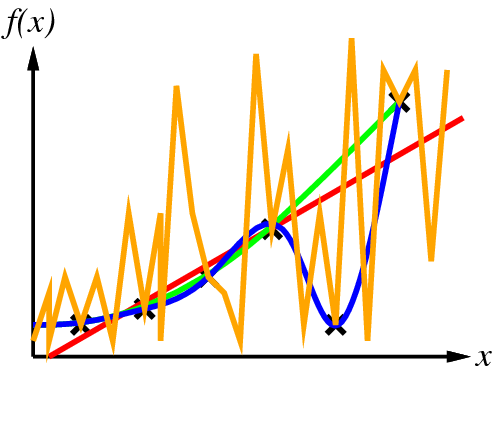
\includegraphics[width=5cm]{./images/curve-fitting5.png}
		\end{center}
	\end{answer}
	\item  In the context of machine learning, explain what is meant by the term \textbf{inductive bias} and illustrate your explanation using examples of inductive biases used by machine learning algorithms.
	\marks{15}
	\begin{answer}
		\begin{itemize}
				\item The inductive bias of a learning algorithm:
				\begin{enumerate}
					\item is a set of assumptions about what the true function we are trying to model looks like.
					\item defines the set of hypotheses that a learning algorithm considers when it is learning.
					\item guides the learning algorithm to prefer one hypothesis (i.e. the hypothesis that best fits with the assumptions) over the others. 
					\item is a necessary prerequisite for learning to happen because inductive learning is an ill posed problem. 
				\end{enumerate}	
				\item Examples of the specific inductive bias introduced by particular machine learning algorithms, include:		
				\begin{itemize}
					\item Maximum margin: when drawing a boundary between two classes, attempt to maximize the width of the boundary. This is the bias used in Support Vector Machines. The assumption is that distinct classes tend to be separated by wide boundaries.
					\item Minimum cross-validation error: when trying to choose among hypotheses, select the hypothesis with the lowest cross-validation error.
				\end{itemize}
			\end{itemize}
	\end{answer}

	\item Explain what can go wrong when a machine learning classifier uses the wrong inductive bias.
	\marks{5}
\begin{answer}
			\begin{itemize}
				\item If the inductive bias of the learning algorithm constrains the search to only consider simple hypotheses we may have excluded the real function from the hypothesis space. In other words, the true function is \textbf{unrealizable} in the chosen hypothesis space, (i.e., we are \textbf{underfitting}). 
				\item If the inductive bias of the learning algorithm allows the search to consider complex hypotheses, the model may hone in on irrelevant factors in the training set. In other words the model with \textbf{overfit} the training data.
			\end{itemize}
\end{answer}


\end{enumerate}


\newpage

%Q2
% knn and CBR 
% information theory, entropy, Decision Trees, Inductive logic programming

\newpage

\question 
	\begin{enumerate}
		\item A data analyst building a \emph{k}-nearest neighbour model for a continuous prediction problem is considering appropriate values to use for $k$. 
	\begin{enumerate}
		\item Initially the analyst uses a simple average of the target variables for the $k$ nearest neighbours in order to make a new prediction. After experimenting with values for $k$ in the range $0 - 10$ it occurs to the analyst that they might get very good results if they set $k$ to the total number of instances in the training set. Do you think the analyst is likely to get good results using this value for $k$?
		\marks{5}
\begin{answer}
In answering this question students should realise that if the analyst set $k$ to the number of training examples all predictions would essentially be the average target value across the whole dataset. To score very well students should realise that this is an example of massive underfitting.
\end{answer}
		\item If the analyst was using a distance weighted averaging function rather than a simple average for their predictions would this have made their idea any more useful?
		\marks{5}
\begin{answer}
Students should realise that yes, if distance weighted voting is used (particularly if a $\frac{1}{d^2}$ type distance weight is used) then examples that are far away from the query will have very little impact on the result. Again to score well students should mention that when distance weighted voting is used the value of $k$ in $k$-NN classifiers is much less important.
\end{answer}
	\end{enumerate}
		\item A dataset showing the decisions made by an individual about whether to wait for a table at a restaurant is listed in Table 1 on the next page. (Note that Table \ref{tab:info-eqs}, also on the next page, lists some equations that you may find useful for this question.)		
	\begin{enumerate}
		\item Given that the $WillWait$ column lists the values of the target variable, compute the entropy for this dataset.
			\marks{5}
			\begin{answer}
					There are 6 positive and 6 negative examples in this dataset. This means that the entropy for the dataset is:
					\begin{eqnarray*}
						I(\frac{6}{12}, \frac{6}{12}) &=& -\frac{6}{12}\log_2\frac{6}{12} + -\frac{6}{12}\log_2 \frac{6}{12}\\
									~ &=& (-\frac{1}{2}\log_2\frac{1}{2}) + (-\frac{1}{2}\log_2\frac{1}{2}) \\ 
						~ &=&  -\frac{1}{2}(-1) + -\frac{1}{2}(-1) \\
						 ~ &=&  1bit
					\end{eqnarray*}			
			\end{answer}
		\item What is the information gain for the $Patrons$ feature?
			\marks{5}
			\begin{answer}
							$Gain(Patrons)=1- ( \frac{2}{12}I(0,1) + \frac{4}{12}I(1,0) + \frac{6}{12}I(\frac{2}{6},\frac{4}{6}) ) \approx 0.541$ bits
			\end{answer}
		\item What is the information gain for the $Type$ feature?
			\marks{5}
			\begin{answer}
							$Gain(Type)=1- ( \frac{2}{12}I(\frac{1}{2},\frac{1}{2}) + \frac{1}{2}I(\frac{1}{2},\frac{1}{2}) + \frac{4}{12}I(\frac{2}{4},\frac{2}{4})+ \frac{4}{12}I(\frac{2}{4},\frac{2}{4}) ) = 0$ bits
			\end{answer}
		\item Given a choice between the $Patrons$ and $Type$ feature, which feature would the ID3 algorithm choose as the root node for a decision tree?
			\marks{5}
			\begin{answer}
					The ID3 algorithm would choose the Patrons feature as the root node for the decision tree because it has the higher information gain.
			\end{answer}
	\end{enumerate}
\end{enumerate}

\newpage 

\begin{table}[h]
%\begin{tiny}
\begin{center}
\begin{tabular}{|l||c|c|c|c|c|c|c||c|}
\hline
%\textbf{Example} & \multicolumn{5}{c||}{\textbf{Attributes}} & \textbf{Target} \\ 
%\cline{2-6}
 ID & $Bar$ & $Patrons$ & $Price$ & $Rain$ & $Type$ & WillWait \\
\hline
$1$  & F & Some & \$\$\$ & F & French &  $T$\\
$2$    & F & Full & \$ & F & Thai &  $F$\\
$3$    & T & Some & \$ & F & Burger &  $T$\\
$4$    & F & Full & \$ & F & Thai  &  $T$\\
$5$    & F & Full & \$\$\$ & F & French &  $F$\\
$6$    & T & Some & \$\$ & T & Italian &  $T$\\
$7$    & T & None & \$ & T & Burger &  $F$\\
$8$    & F & Some & \$\$ & T & Thai &  $T$\\
$9$     & T & Full & \$ & T & Burger &  $F$\\
$10$ & T & Full & \$\$\$ & F & Italian &  $F$\\
$11$ & F & None & \$ & F & Thai &  $F$\\
$12$ & T & Full & \$ & F & Burger &  $T$\\
\hline
\end{tabular}
\end{center}
%\end{tiny}
\label{tab:rest}
\caption{A dataset describing the previous decisions made by an individual about whether to wait for a table at a restaurant.}
\end{table}

	\begin{table}[htb]
	\begin{center}
	\begin{tabular}{rl}
	Entropy(DS) & $\displaystyle = -\sum_{i=1}^k p_i \times log_2(p_i)$\\
	Remainder(F) & $\displaystyle =\sum_{v \in Domain(F)} \frac{|DS_v|}{|DS|} Entropy(DS_v)$\\
	InformationGain(F,DS) & $\displaystyle =Entropy(DS)-Remainder(F)$\\
	\end{tabular}
	\end{center}
	\caption{Equations from information theory.}
	\label{tab:info-eqs}
	\end{table}

\newpage

			

	
%Q3 30 marks
% basic probability 5
% bayesian networks 10
% bayesian learning  15

\question Table \ref{tab:spamhamdata} (on the next page) lists a dataset of the subject lines from emails. Table \ref{tab:spamhamquery} (also on the next page) shows the subject line for an email that we would like to classify as Spam or Ham. 
	\begin{enumerate}
		\item Using \textbf{Laplacian smoothing}, where 
		\begin{eqnarray*}
		p(x=v) &=& \frac{count(x=v)+k}{count(x) +( k \times |Domain(x)|)}
		\end{eqnarray*}
		with \textbf{k=1} and a \textbf{vocabulary size of 12}, calculate the following probabilities:
			\begin{enumerate}
				\item $P(Spam)=?$
				\marks{2}
					\begin{answer}
						$P(Spam) = \frac{3+1}{8 + (1 \times 2)} = \frac{4}{10} = 0.4$
					\end{answer}
				\item $P(Ham)=?$
				\marks{2}
					\begin{answer}
						$P(Ham) = \frac{5+1}{8 + (1 \times 2)} = \frac{6}{10} = 0.6$
					\end{answer}
				\item $P('Fun'|Spam)=?$
				\marks{2}
					\begin{answer}
						$P('Fun'|Spam) = \frac{0+1}{9 + (1 \times 12)} = \frac{1}{21} = 0.0476$
					\end{answer}
				\item $P('Fun'|Ham)=?$
				\marks{2}
					\begin{answer}
						$P('Fun'|Ham) = \frac{2+1}{15 + (1 \times 12)} = \frac{3}{27} = 0.1111$
					\end{answer}
				\item $P('is'|Spam)=?$
				\marks{2}
					\begin{answer}
						$P('is'|Spam) = \frac{1+1}{9 + (1 \times 12)} = \frac{2}{21} = 0.0952$
					\end{answer}
				\item $P('is'|Ham)=?$
				\marks{2}
					\begin{answer}
						$P('is'|Ham) = \frac{1+1}{15 + (1 \times 12)} = \frac{2}{27} = 0.0741$
					\end{answer}
				\item $P('Free'|Spam)=?$
				\marks{2}
					\begin{answer}
						$P('Free'|Spam) = \frac{3+1}{9 + (1 \times 12)} = \frac{4}{21} = 0.1905$
					\end{answer}
				\item $P('Free'|Ham)=?$
				\marks{2}
					\begin{answer}
						$P('Free'|Ham) = \frac{1+1}{15 + (1 \times 12)} = \frac{2}{27} = 0.0741$
					\end{answer}
			\end{enumerate}
		\item Calculate the probability of the query title in Table \ref{tab:spamhamquery} belonging to the Spam class under the \textbf{Naive Bayes assumption} and using the \textbf{smoothed probabilities} you calculated in Part (a):		
%Using the smoothed probabilities you calculated in Part 1 of calculate the probability under the \textbf{Naive Bayes assumption} of the query title in Table \ref{tab:songmoviequery} belonging to the Movie class:
			\begin{center}
				$P(Spam|'Fun~is~Free')=?$
			\end{center}
			\marks{7}
			\begin{answer}
				$P(Spam|'Fun is Free')$ 
				\begin{scriptsize}
				\begin{eqnarray*}
					&=& \frac{P('Fun'|Spam)P('is'|Spam)P('Free'|Spam)P(Spam)}{(P('Fun'|Spam)P('is'|Spam)P('Free'|Spam)P(Spam))+(P('Fun'|Ham)P('is'|Ham)P('Free'|Ham)P(Ham))}\\
					&=& \frac{0.0476 \times 0.0952 \times 0.1905 \times 0.4}{(0.0476 \times 0.0952 \times 0.1905 \times 0.4) + (0.1111 \times 0.0741 \times  0.0741 \times 0.6)}\\
					&=& 0.48543863
				\end{eqnarray*}
				\end{scriptsize}
			\end{answer}
		\item Calculate the probability of the query title in Table \ref{tab:spamhamquery} belonging to the Spam class under the \textbf{Naive Bayes assumption} and using \textbf{maximum likelihood} probabilities (i.e. the probabilities we could get if we did not use Laplacian smoothing):	
%Using \textbf{maximum likelihood} probabilities (i.e. do not use Laplacian smoothing in calculating the probabilities) calculate the probability under the \textbf{Naive Bayes assumption} of the query title in Table \ref{tab:songmoviequery} belonging to the Movie class:	
					\begin{center}
				$P(Spam|'Fun~is~Free')=?$
			\end{center}
			\marks{7}
			\begin{answer}
				Because the word 'Fun' does not appear in any of the Spam titles the maximum likelihood (i.e., unsmoothed) probability of $P('Fun'|Spam)=0$. As a result the maximum likelihood probability of $P(Spam|'Fun~is~Free')=0$. Showing the complete calculation: \\
				\\
				P(Spam|'Fun~is~Free')
				\begin{scriptsize}
				\begin{eqnarray*}
					&=& \frac{P('Fun'|Spam)P('is'|Spam)P('Free'|Spam)P(Spam)}{(P('Fun'|Spam)P('is'|Spam)P('Free'|Spam)P(Spam))+(P('Fun'|Ham)P('is'|Ham)P('Free'|Ham)P(Ham))}\\
					&=& \frac{\frac{0}{9} \times \frac{1}{9} \times \frac{3}{9} \times \frac{3}{8}}{(\frac{0}{9} \times \frac{1}{9} \times \frac{3}{9} \times \frac{3}{8})+(\frac{2}{15} \times \frac{1}{15} \times \frac{1}{15} \times \frac{5}{8})}\\
					&=& 0.0
				\end{eqnarray*}
				\end{scriptsize}
			\end{answer}
	\end{enumerate}

\newpage

\begin{table}[!htb]
    \caption{Spam and Ham Dataset}
    \begin{minipage}{.5\linewidth}
      \centering
\begin{tabular}{l}
\textbf{Spam}\\
\hline
\textit{Offer is Free}\\
\textit{Free Learning Link}\\
\textit{Cick Free Link}\\
\hline
\end{tabular}
    \end{minipage}%
    \begin{minipage}{.5\linewidth}
      \centering
\begin{tabular}{l}
\textbf{Ham}\\
\hline
\textit{Great Learning Fun}\\
\textit{Great Machine Learning}\\
\textit{Free Learning Event}\\
\textit{Learning is Fun}\\
\textit{Learning Costs Money}\\
\hline
\end{tabular}
    \end{minipage} 
    \label{tab:spamhamdata}
\end{table}

\begin{table}[h]
\caption{Query Title}
\centering
\begin{tabular}{l}
\hline
\textit{Fun is Free}\\
\hline
\end{tabular}
\label{tab:spamhamquery}
\end{table}



\newpage

%Q4
%Linear Regression Neural Nets, SVMs, Ensemble Learning

\begin{table}
\begin{center}
\begin{tabular}{cccccc}
\hline
x & 0 & 1 & 2 & 3 & 4\\
\hline
y & 3 & 6 & 7 & 8 & 11\\
\hline
\end{tabular}
\caption{Example Dataset for Linear Regression Question}
\label{tab:linregTab2}
\end{center}
\end{table}

\question 
	\begin{enumerate}
		%Regression Learning
		\item Assuming a domain with one descriptive feature $x$ and one target feature $y$, linear regression uses the following formula to model the relationship between the descriptive and target features: 
	\begin{center}
		$\displaystyle f(x) = w_1x + w0$
	\end{center}
where $w1$ and $w0$ are computed using the following formulae, where $M$ is number of data points in the dataset:
	\begin{center}
		$\displaystyle w_1 =  \frac{(M \sum_{i=1}^M x_i y_i) - (\sum_{i=1}^{M} x_i \sum_{i=1}^{M} y_i)} {(M \sum_{i=1}^{M} x_i^2) - (\sum_{i=1}^{M} x_i)^2}$
	\end{center}
	\begin{center}
		$\displaystyle w_0 = (\frac{1}{M} \sum_{i=1}^{M} y_i) - (\frac{w_1}{M} \sum_{i=1}^{M} x_i)$
	\end{center}
Using the data in Table \ref{tab:linregTab2} compute the values of $w_0$ and $w_1$ that provide the best linear fit to the data.
			\marks{10}
			\begin{answer}
				First we need to compute the values of the equation components:
			\begin{itemize}
				\item M = 5
				\item $\sum_{i=1}^{M} x_i y_i = 0 + 6 + 14 + 24 + 44 = 88$
				\item $\sum_{i=1}^{M} x_i = 10$
			   	\item $\sum_{i=1}^{M} y_i = 35$
			  	\item $\sum_{i=1}^{M} x_i^2 = 0 + 1 + 4 + 9 + 16 = 30$
			  	\item $(\sum_{i=1}^{M} x_i)^2 = 10^2 = 100$
			\end{itemize}
				Given these values,  $w_1$:
				\begin{center}
					\textbf{$w_1= \frac{(5*88)-(10*35)}{(5*30)-100} = \frac{90}{50}=1.8$}
				\end{center}
				And, $w_0$:
				\begin{center}
				\textbf{$w_0= (\frac{1}{5}*35) - (\frac{1.8}{5}*10)= 7-3.6=3.4$}
			\end{center}
			\end{answer}
		
		%Neural Nets	
		\item Figure \ref{fig:nn} (on the next pages) shows a backprogation network that is currently processing the training vector $[1.0, 0.9, 0.9]$ which has an  associated target vector $[0.1, 0.9, 0.1]$. Given that the output from unit B is $0.6$ and from C is $0.8$, and assuming that the activation function used at all nodes in the network is the logistic function, carry out the calculations listed below. Note that Table \ref{tab:nn-eqs} (also on the next page) lists some equations that you may find useful when doing this question. 
\begin{enumerate}
	\item Calculate the actual output vector (to 3 decimal places).
	\marks{10}
		\begin{answer}
		%Output of unit $x = a_x(in_x) = \frac{1}{1 + \exp^{-\sum_j W_{jx} a_j(in_j)}}\\
		%First output unit input $i$\\
		\begin{eqnarray*}
		a_i(in_i) &=&\frac{1}{1 + \exp^{- ((W_{BD} \times a_B(in_B) + (W_{CD} \times a_C(in_C) ))}}\\
		&=&\frac{1}{1 + \exp^{- ((-0.3 \times 0.6) + (0.9 \times 0.8}))}\\
		&=&\frac{1}{1 + \exp^{- 0.54}}\\
		&=&0.632
		\end{eqnarray*}
		%Second output unit input $j$\\
		\begin{eqnarray*}
		a_j(in_j) &=&\frac{1}{1 + \exp^{- ((W_{BE} \times a_B(in_B) + (W_{CE} \times a_C(in_C) ))}}\\
		& = &\frac{1}{1 + \exp^{- ((-0.6 \times 0.6) + (0.1 \times 0.8}))}\\
		& = &\frac{1}{1 + \exp^{- (-0.44)}}\\
		& = &0.392
		\end{eqnarray*}
		%Third output unit input $k$\\
		\begin{eqnarray*}
		a_k(in_k) &=&\frac{1}{1 + \exp^{- ((W_{BF} \times a_B(in_B) + (W_{CF} \times a_C(in_C) ))}}\\
		& = &\frac{1}{1 + \exp^{- ((0.4 \times 0.6) + (1.2 \times 0.8}))}\\
		& = &\frac{1}{1 + \exp^{- 1.2}}\\
		& = &0.769
		\end{eqnarray*}
		\end{answer}
	\item Calculate the \textbf{$\Delta$} error for each output unit (to 3 decimal places).
	\marks{6}
		\begin{answer}
		\begin{eqnarray*}
		\Delta_D& = &(target_D - a_D(in_D)) \times a_D(in_D) \times (1-a_D(in_D))\\
		& = &(0.1-0.632) \times 0.632 \times (1-0.632)\\
		& = &-0.124
		\end{eqnarray*}
%		Second output unit $j$\\
		\begin{eqnarray*}
		\Delta_E& = &(target_E - a_E(in_E)) \times a_E(in_E) \times (1-a_E(in_E))\\
		& = &(0.9-0.392) \times 0.392 \times (1-0.392)\\
		& = &0.121
		\end{eqnarray*}
%		Third output unit $k$\\
		\begin{eqnarray*}
		\Delta_F& = &(target_F - a_F(in_F)) \times a_F(in_F) \times (1-a_F(in_F))\\
		& = &(0.1-0.769) \times 0.769 \times (1-0.769)\\
		& = &-0.119
		\end{eqnarray*}
		\end{answer}
%	\item Calculate the \textbf{$\Delta$} error for each hidden unit B and C. (to 3 decimal places)\\
%		\begin{answer}
%%Again we are using backprop to train a multi-layer network so we use the Delta error rules. In this case the Delta error rule for hidden units.Each hidden node $j$ is responsible for some fraction of the error $\Delta_i$ of each of the output units $i$ to which it connects. Thus the $\Delta_i$ values are divided according to the strengths of the connection between the hidden node and the output nodes and are propagated back to the hidden nodes. Where a hidden node feeds-forward into more than 1 output node the errors propagated back to it are summed. So the error for a hidden unit $j$ feeding into $n$ units= $\Delta_j = a_j(in_j) \times (1-a_j(in_j)) \times \left( \sum_{i=1}^{n}W_{ji} \times \Delta_i \right)$\\
%
%\begin{eqnarray*}
%\Delta_B &=& a_B(in_B) \times (1-a_B(in_B)) \times \left( \sum_{x \in \{D,E,F\}}^{n}W_{Bx} \times \Delta_x \right)\\
%&=& a_B(in_B) \times (1-a_B(in_B)) \times \left(((W_{BD} \times \Delta_D)+(W_{BE} \times \Delta_E)+(W_{BF} \times \Delta_F))\right)\\
%&=& 0.6 \times (1-0.6) \times \left(((-0.3 \times -0.124)+(-0.6 \times 0.121)+(0.4 \times -0.119))\right)\\
%&\approx& -0.020\\
%\end{eqnarray*}
%
%\begin{eqnarray*}
%\Delta_C &=& a_C(in_C) \times (1-a_C(in_C)) \times \left( \sum_{x \in \{D,E,F\}}^{n}W_{Cx} \times \Delta_x \right)\\
%&=& a_C(in_C) \times (1-a_C(in_C)) \times \left(((W_{CD} \times \Delta_D)+(W_{CE} \times \Delta_E)+(W_{CF} \times \Delta_F))\right)\\
%&=& 0.8 \times (1-0.8) \times \left(((0.9 \times -0.124)+(-0.1 \times 0.121)+(1.2 \times -0.119))\right)\\
%&\approx& -0.043\\
%\end{eqnarray*}
%
%		\end{answer}
	\item Calculate the new weight $W_{BD}$ for the connection from unit B to the output unit D after the training example has been processed. Use a learning rate of $\eta = 0.25$.
		\marks{4}
		\begin{answer}
		\begin{eqnarray*}			
		W_{B,D} &=& W_{B,D} + (\eta \times a_B(in_B) \times \Delta_D)\\
				&=& -0.3 + (0.25 \times 0.6 \times -0.124)\\
		           &=& -0.319
		\end{eqnarray*}
	\end{answer}
\end{enumerate}

\end{enumerate}

\clearpage
\newpage

\begin{figure}[htbp]
\begin{center}
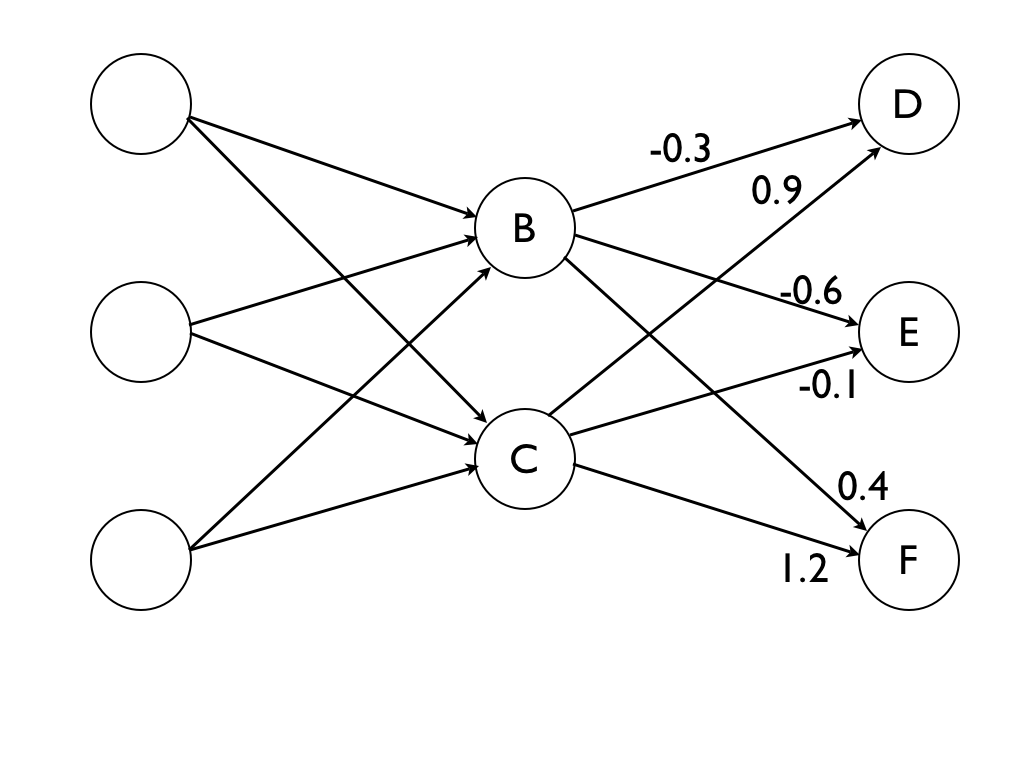
\includegraphics[width=3.5in]{./images/backpropnetwork1.png}
\caption{Example Neural Net}
\label{fig:nn}
\end{center}
\end{figure}

	\begin{table}[htb]
	\begin{center}
	\begin{tabular}{ll}
	Weighted sum of inputs for unit $i$ with $j$ inputs:  & $\displaystyle in_i = \sum_j W_{ji} a_j(in_j)$\\
	Activation Function (Logistic) for unit $i$: & $\displaystyle a_i(in_i) = \frac{1}{1 + \exp^{-in_i}}$ \\
	Perceptron weight update rule for link  $j\rightarrow i$ & $\displaystyle w_{ji}=w_{ji} + \eta \left( t_i - a_i(in_i) \right) \times a_j(in_j)$\\
      Hebbian Weight Update Rule for link  $j\rightarrow i$ & $\displaystyle w_{ji} = \eta \times a_j(in_j) \times a_i(in_i)$\\
	Partial Derivative for Logistic Activation Function & $\displaystyle \frac{\delta a_i(in_i)}{\delta in_i}=a_i(in_i) \times (1-a_i(in_i))$\\
	Error for an output unit $i$ & $\displaystyle error_i =  target_i - a_i(in_i)$\\
	Delta Error for an output unit $i$ & $\displaystyle \Delta_i =  error_i \times a_i(in_i) \times (1-a_i(in_i))$\\
	Delta Error for a hidden unit $j$ feeding into $n$ units & $\displaystyle \Delta_j = \left( \sum_{i=1}^{n}W_{ji} \times \Delta_i \right) \times a_j(in_j) \times \left(1-a_j(in_j)\right)$\\
      Delta Weight Update Rule for link $x \rightarrow k$ & $\displaystyle W_{x,k} = W_{x,k} + (\eta \times a_x(in_x) \times \Delta_k)$\\
	\end{tabular}
	\end{center}
	\caption{Equations used in Perceptron and Neural Network training.}
	\label{tab:nn-eqs}
	\end{table}


\end{document}
